\documentclass[11pt]{article}

\usepackage[T1]{fontenc}
\usepackage[utf8]{inputenc}
\usepackage{lmodern}
\usepackage[margin=1in]{geometry}
\usepackage{microtype}
\usepackage{graphicx}
\usepackage{booktabs}
\usepackage{tabularx}
\usepackage{array}
\usepackage{amsmath}
\usepackage{float}
\usepackage{xcolor}
\usepackage{url}
\usepackage[numbers,sort&compress]{natbib}
\usepackage[hidelinks]{hyperref}

\graphicspath{{images/}}
\setlength{\emergencystretch}{2em}
\renewcommand{\arraystretch}{1.12}

\title{The Renewable Grid, Hour by Hour}
\author{Shazab Ali}
\date{Final academic report\\Data period: January 1--December 31, 2025}

\begin{document}
\maketitle

\begin{center}
\textbf{Source code:} \url{https://github.com/shaz1234567/renewable-grid-story}\\
\textbf{Working visualization:} \url{https://renewable-grid-story.onrender.com/}
\end{center}

\begin{abstract}
This project is a six-view interactive scientific story about how solar, wind, and hydropower vary through a day, across a year, and among four U.S.\ balancing authorities: California ISO (CISO), Electric Reliability Council of Texas (ERCO), New York ISO (NYIS), and PJM. The Plotly Dash application uses 35,040 hourly authority records derived from U.S.\ Energy Information Administration (EIA) Form 930 for 2025. It combines daily generation-mix context, hourly playback, annual source profiles, matched-period regional comparisons, variability statistics, and renewable-portfolio analysis. Annual renewable energy and shares of net generation were 90.819 million MWh and 48.744\% for CISO, 182.821 million MWh and 37.583\% for ERCO, 31.137 million MWh and 23.500\% for NYIS, and 72.299 million MWh and 8.255\% for PJM. Validation passed 10 of 11 checks. Coverage, timestamps, provenance, and aggregation arithmetic passed, but the dataset contains \textbf{31 missing renewables rows and 31 missing generation-mix rows}; validation is therefore not described as entirely clean. Automated tests cover 20 cases. One documented visual review produced a title/legend readability revision; broader target-audience comprehension testing remains pending.
\end{abstract}

\section{Introduction}
\subsection{Research question}
How can an interactive visual narrative make the temporal and regional differences among solar, wind, and hydropower understandable without hiding scale, variability, missing data, or the limits of descriptive comparisons?

\subsection{Audience}
The primary audience is university students and instructors who understand basic charts but may not know electricity-system terminology. A secondary audience is an interested public reader seeking a concise, evidence-based introduction to balancing-authority generation patterns. The application explains units, limits causal claims, exposes missingness, and presents both absolute and normalized scales.

\subsection{Objectives}
\begin{enumerate}
  \item Show an ordinary operating day in the context of the full reported generation mix.
  \item Let a reader reveal one renewable source hour by hour rather than seeing only a completed line.
  \item Expose annual and seasonal structure using daily means.
  \item Compare the same source and date interval across two authorities, in raw MW or normalized form.
  \item Quantify mean, extrema, sample standard deviation, coefficient of variation (CV), and missing hours.
  \item Test whether a selected renewable portfolio is steadier relative to its mean than its component sources.
  \item Preserve source gaps and disclose methodological boundaries instead of implying forecast or causal evidence.
\end{enumerate}

\subsection{Proposal alignment and documented changes}
The submitted proposal was approved with the instructor comment \textbf{``approved''} and no requested revisions. The implementation preserves the approved central question, 2025 scope, four balancing authorities, three renewable source families, and six-view storyboard. Five justified implementation changes retain that scientific intent:
\begin{enumerate}
  \item Because EIA API-key registration returned ``access denied,'' acquisition uses key-free, versioned EIA-930 bulk archives with recorded checksums.
  \item The 2025 schema splits solar and wind into categories with and without integrated storage. The pipeline combines each source family, uses hydro excluding pumped storage, and excludes standalone and pumped storage.
  \item Plotly Dash was selected from the proposed Plotly/D3 options to support coordinated Python callbacks and reproducible figure tests.
  \item The geographic view uses approximate reference points rather than unsupported balancing-authority polygons.
  \item Source-reported missing values remain visible gaps with notices instead of being converted to zero.
\end{enumerate}

\section{Related Work}
EIA Form 930 provides hourly and daily balancing-authority operating statistics and is the empirical foundation of this project \citep{eia930,eia-gridmonitor}. The downloadable archives used here are a versioned Catalyst Cooperative/PUDL publication on Zenodo, supporting reproducible provenance through published checksums and a fixed record version \citep{pudl-zenodo}. The EIA balancing-authority overview supplies institutional context for interpreting CISO, ERCO, NYIS, and PJM as operating regions rather than state boundaries.

The interaction design follows an overview-to-detail sequence: begin with context, provide filters and matched comparisons, and reveal exact values through hover and metric cards. Plotly and Dash provide declarative charts and controls \citep{plotly,dash}. Normalization is never presented as energy share: each selected series is divided by its own peak, so it answers when a profile rises and falls, not how large the system is. This work is an explanatory visualization, not a forecasting model, dispatch simulation, or causal study.

\section{Methodology and Workflow}
\subsection{Data source and provenance}
The source is the \textit{EIA Form 930 Hourly and Daily Balancing Authority Operations Report}. The project uses version 97.0.0 of the Catalyst Cooperative/PUDL archive \citep{pudl-zenodo}: \texttt{eia930-2025half1.zip} (264,934 source rows) and \texttt{eia930-2025half2.zip} (267,218 source rows). The raw manifest records published MD5 values and locally verified SHA-256 hashes. Validation confirms that both archives exist and match the recorded integrity values.

\subsection{Processed schema and sample records}
Filtering to CISO, ERCO, NYIS, and PJM produces 35,040 records: 8,760 local operating-date rows per authority. The 24-column Parquet schema contains identifiers, local and UTC dates, demand and net generation, reported fuel columns, and derived solar, wind, renewable, and generation-mix fields.

\begin{table}[H]
\centering
\caption{Illustrative processed CISO records from January 1, 2025.}
\label{tab:samples}
\small
\begin{tabular}{l l l r r r r r}
\toprule
BA & Local hour end & UTC hour end & Solar & Wind & Hydro & Renew. & Mix \\
 & & & \multicolumn{5}{c}{MW} \\
\midrule
CISO & Jan.\ 1 01:00 & Jan.\ 1 09:00Z & -52 & 664 & 2,581 & 3,193 & 15,113 \\
CISO & Jan.\ 1 02:00 & Jan.\ 1 10:00Z & -52 & 465 & 2,241 & 2,654 & 14,534 \\
CISO & Jan.\ 1 03:00 & Jan.\ 1 11:00Z & -52 & 332 & 2,179 & 2,459 & 14,035 \\
\bottomrule
\end{tabular}
\end{table}

Negative reported values are retained; they are not silently clipped in the data or charts.

\subsection{Preparation and transformations}
For every source field, preparation uses the first numeric value available in this order: adjusted, imputed, then raw. Dates are parsed into a local operating date, local end-of-hour timestamp, and timezone-aware UTC timestamp. Records are sorted by authority and UTC timestamp and written as compressed Parquet. Solar and wind combine reported components:
\begin{align}
\mathrm{Solar}_t &= \mathrm{SolarWithoutBattery}_t+\mathrm{SolarWithBattery}_t,\\
\mathrm{Wind}_t &= \mathrm{WindWithoutBattery}_t+\mathrm{WindWithBattery}_t.
\end{align}
If an integrated-storage component is entirely unreported, it remains nullable in its source column but contributes zero when another component is present. Primary renewables are
\begin{equation}
\mathrm{Renewables}_t=\mathrm{Solar}_t+\mathrm{Wind}_t+\mathrm{Hydro}_t,
\end{equation}
where hydropower excludes pumped storage. The generation mix is
\begin{align}
\mathrm{Mix}_t={}&\mathrm{Coal}_t+\mathrm{NaturalGas}_t+\mathrm{Nuclear}_t+\mathrm{Petroleum}_t \nonumber\\
&+\mathrm{Hydro}_t+\mathrm{Solar}_t+\mathrm{Wind}_t+\mathrm{Geothermal}_t
+\mathrm{Other}_t+\mathrm{Unknown}_t.
\end{align}
Standalone battery storage, pumped storage, other storage, and unknown storage are excluded. Since each observation is a one-hour average,
\begin{equation}
\mathrm{Energy\ (MWh)}=\sum_{t=1}^{n}\mathrm{MW}_t\times 1\ \mathrm{hour}.
\end{equation}
Daily charts use the mean of available hourly observations:
\begin{equation}
\bar{x}_{\mathrm{day}}=\frac{1}{n_{\mathrm{available}}}\sum_t x_t.
\end{equation}
Renewable share and independently normalized profiles are
\begin{align}
\mathrm{Share}_{\mathrm{renewable}}&=100\frac{\sum_t\mathrm{Renewables}_t}{\sum_t\mathrm{NetGeneration}_t},\\
\mathrm{Normalized}_t&=100\frac{x_t}{\max_t|x_t|}.
\end{align}
Variability uses the sample standard deviation:
\begin{equation}
\mathrm{CV}=\frac{s}{|\bar{x}|}.
\end{equation}
CV is undefined when the mean is zero or unavailable. A portfolio is the row-wise sum of selected renewable sources, followed by the same CV calculation.

\subsection{Missing-data handling}
Missing source values remain gaps. Aggregations use available observations and a minimum count of one, so an entirely missing group does not become a false zero. Quality output records 25 missing demand values, 25 missing net-generation values, and \textbf{31 missing values each for solar, wind, hydropower, renewables, and generation mix}. Those 31 renewable/mix gaps occur across ERCO (24), NYIS (6), and PJM (1); CISO has none for the three primary renewable series. Structural non-reporting is also visible: NYIS solar is reported as zero for available rows, while some integrated-storage and unknown-fuel columns can be entirely null.

\subsection{Reproducible workflow}
The implemented sequence is: download two fixed Zenodo archives and verify checksums; record source metadata; filter and transform the four authorities; write data-quality, validation, annual, and monthly metric files; construct six Dash views from read-only Parquet data; export six default-view screenshots; run tests and browser checks; and build the academic outputs.

\section{Six-View Construction and Rationale}
\subsection{View 1: What powers an ordinary day?}
A stacked area chart shows all nonempty reported sources for one authority and date. This prevents renewable output from being interpreted without the rest of the system. On the default CISO date, June 15, solar has the largest summed hourly average: 199,159 MWh-equivalent over 24 records, about 35.1\% of the positive reported mix.
\begin{figure}[H]
\centering
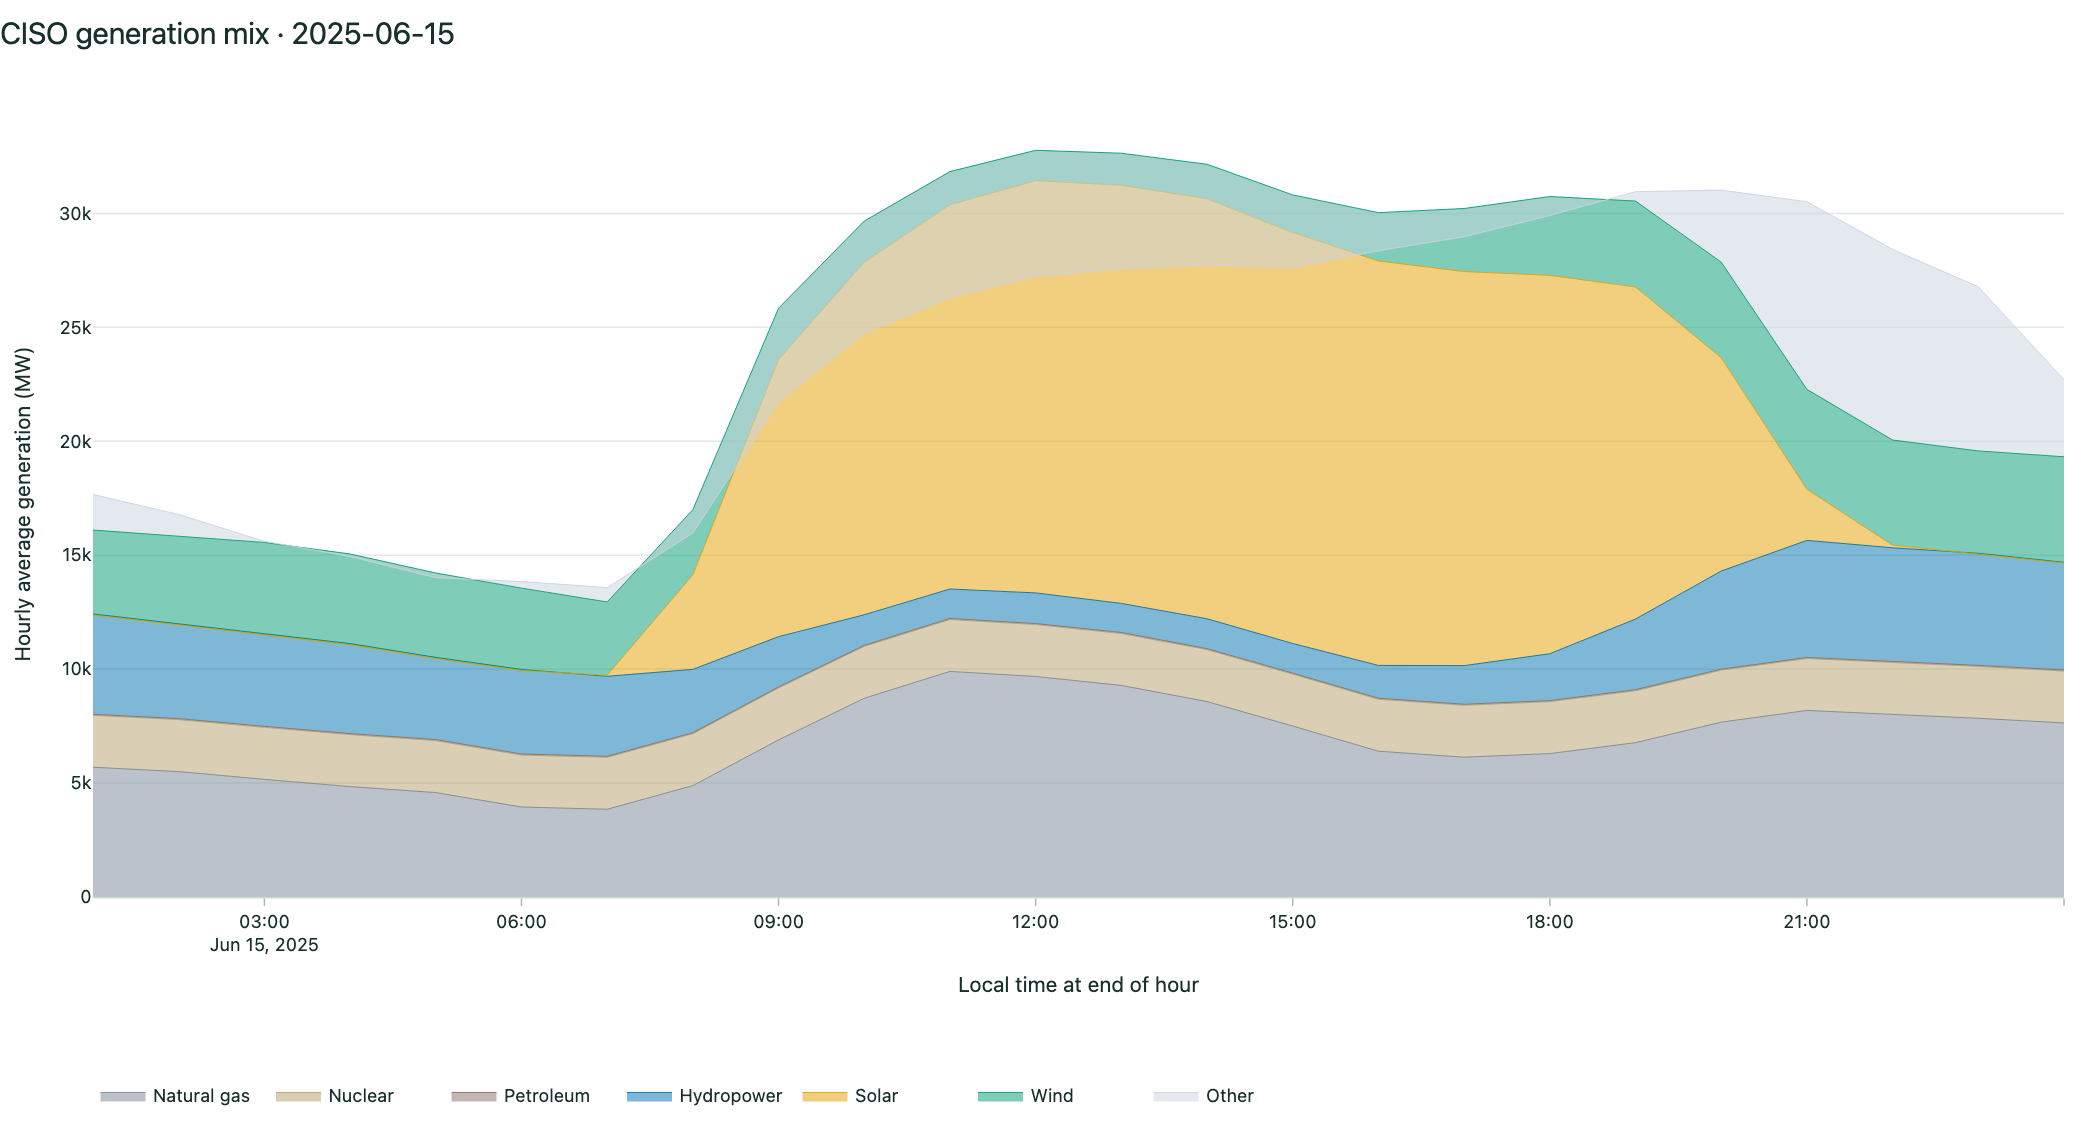
\includegraphics[width=\textwidth]{view-1-generation-mix.png}
\caption{CISO generation mix on June 15, 2025. Negative reports and gaps are retained.}
\label{fig:view1}
\end{figure}

\subsection{View 2: Watch renewables build a day}
Previous, Play/Pause, Next, Reset, and an hour slider reveal one renewable observation at a time. The maximum is derived from the selected day, so 23- and 25-observation daylight-saving days are supported.
\begin{figure}[H]
\centering
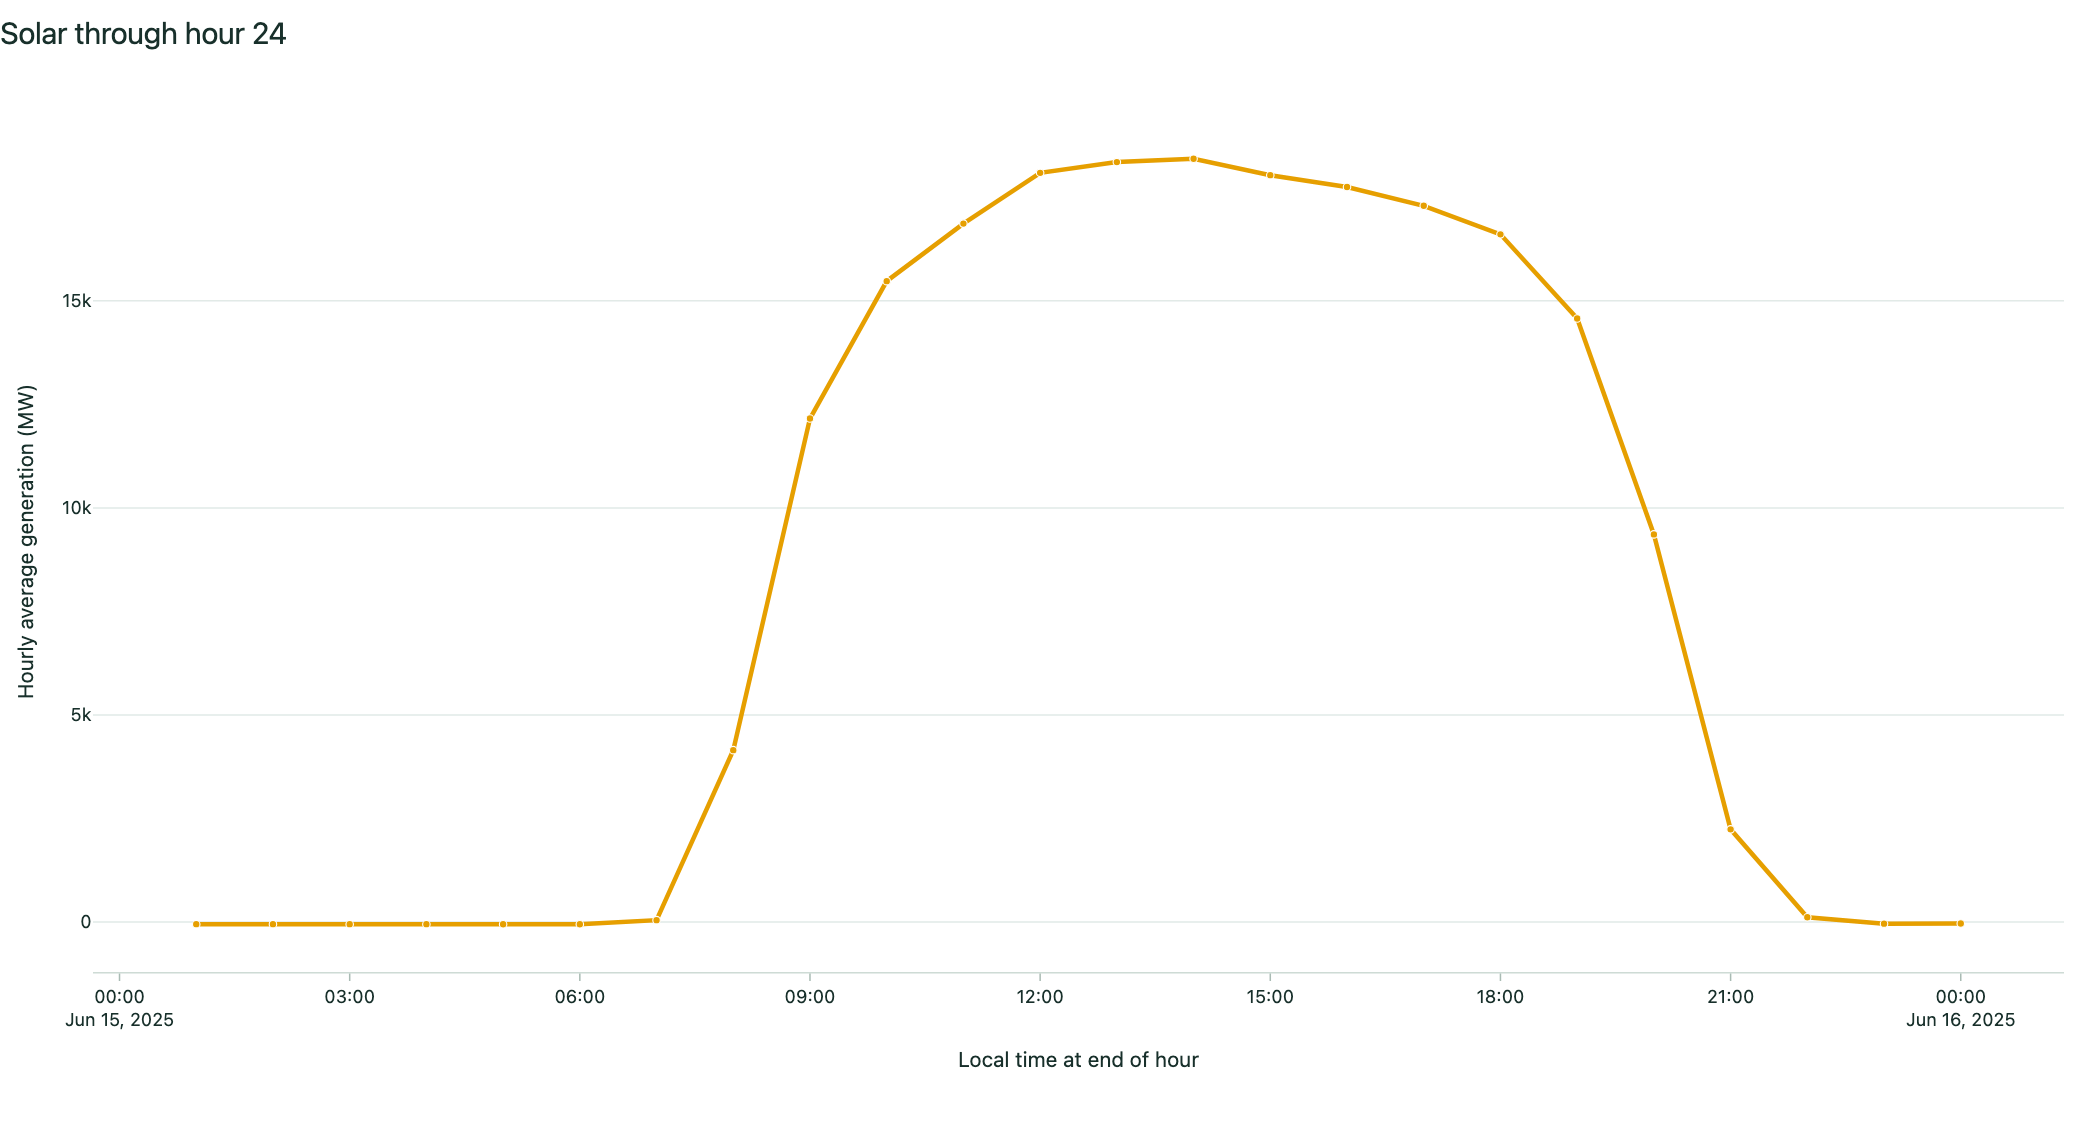
\includegraphics[width=\textwidth]{view-2-hourly-rhythm.png}
\caption{CISO solar revealed hour by hour for June 15, 2025.}
\label{fig:view2}
\end{figure}

\subsection{View 3: Seasons reshape every source}
Daily means reduce 8,760 hourly values into a readable annual pattern. Absolute mode preserves MW scale; normalized mode sets each source's annual peak to 100\%, enabling shape comparison while removing magnitude.
\begin{figure}[H]
\centering
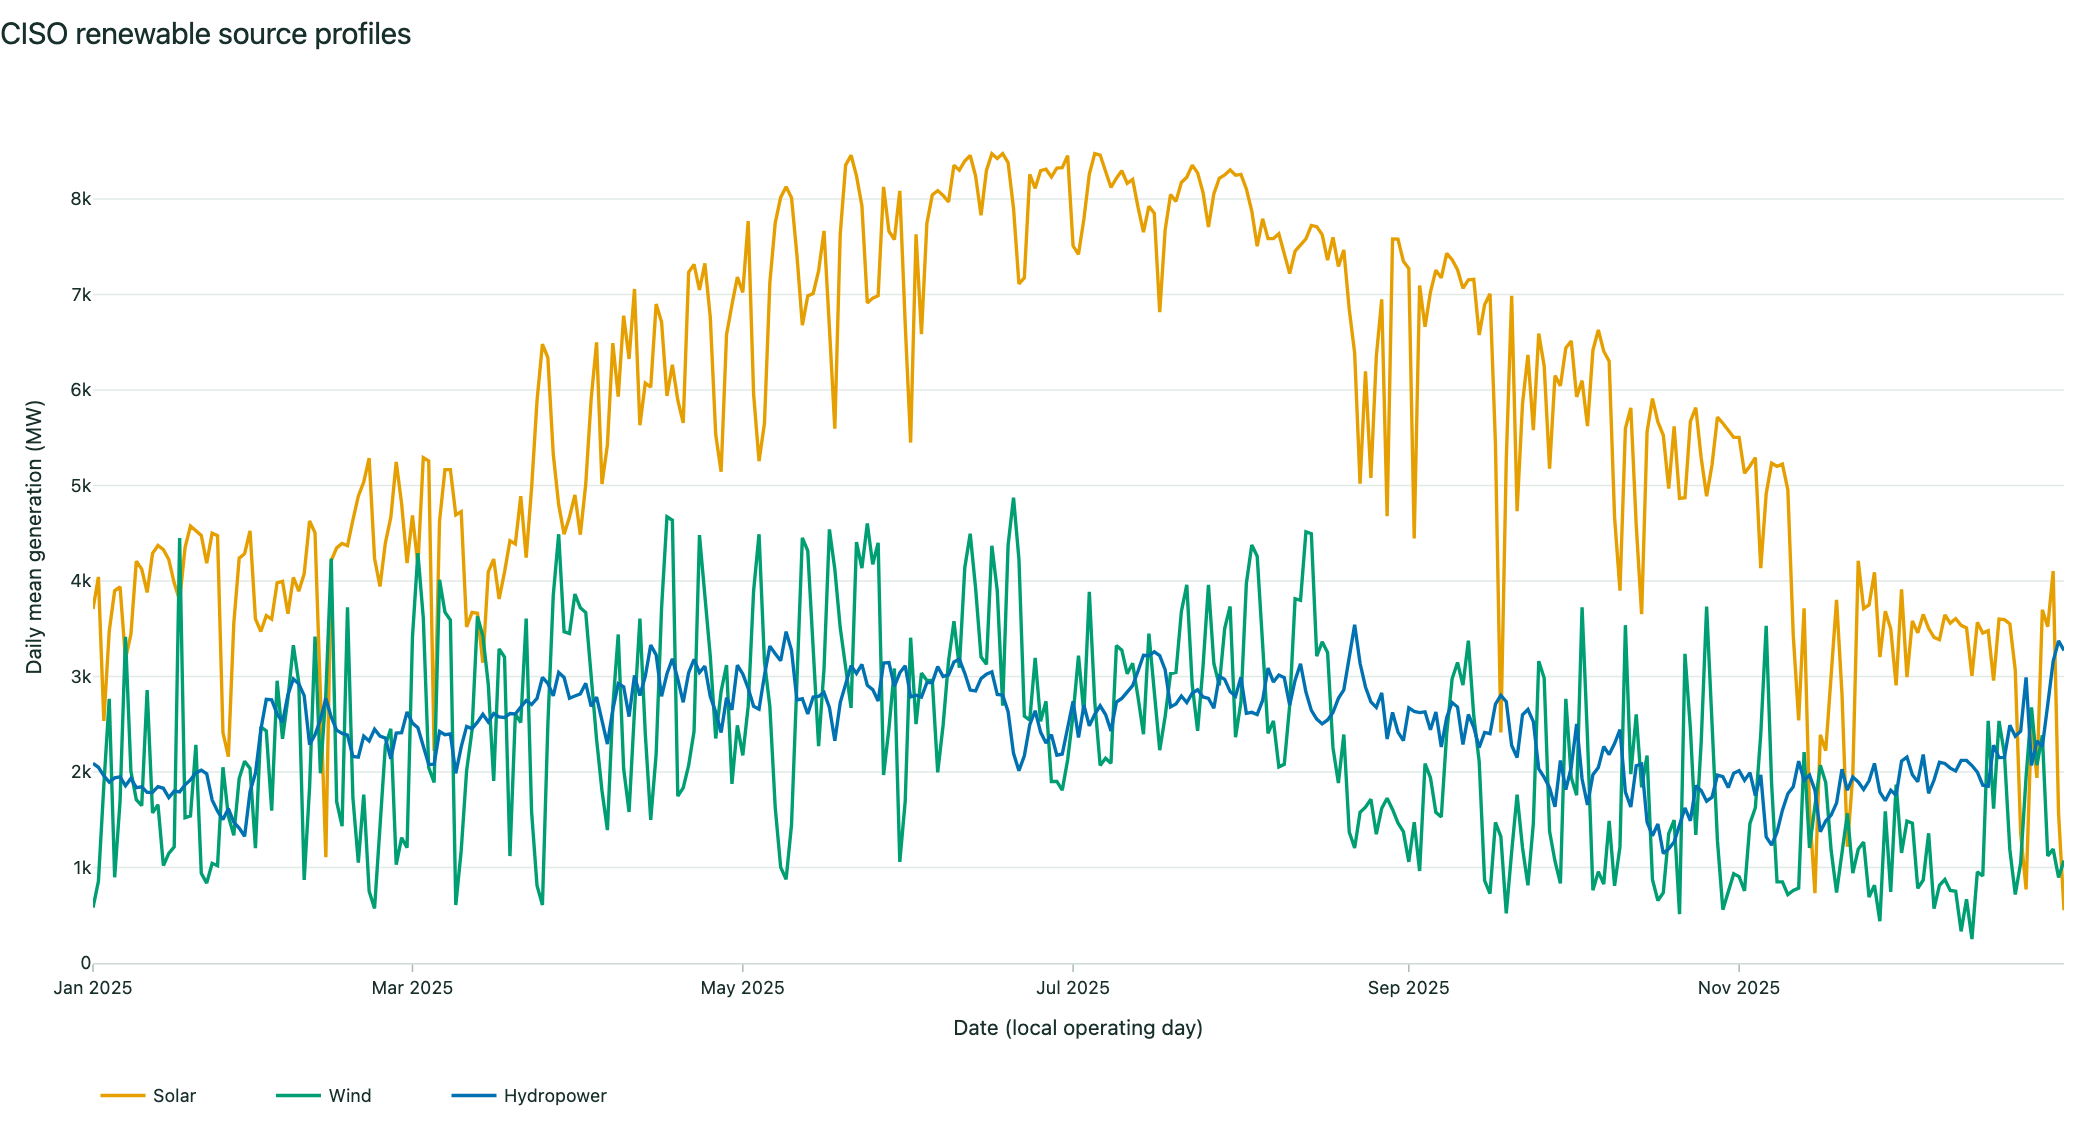
\includegraphics[width=\textwidth]{view-3-source-comparison.png}
\caption{CISO daily-mean solar, wind, and hydropower through 2025.}
\label{fig:view3}
\end{figure}

\subsection{View 4: Place changes the renewable profile}
A schematic U.S.\ map orients readers without claiming balancing-authority boundaries. A paired chart uses the same source and dates for two regions. The default comparison shows ERCO mean solar at about 7,723.9 MW versus CISO at 5,667.9 MW, approximately 1.36 times as high.
\begin{figure}[H]
\centering
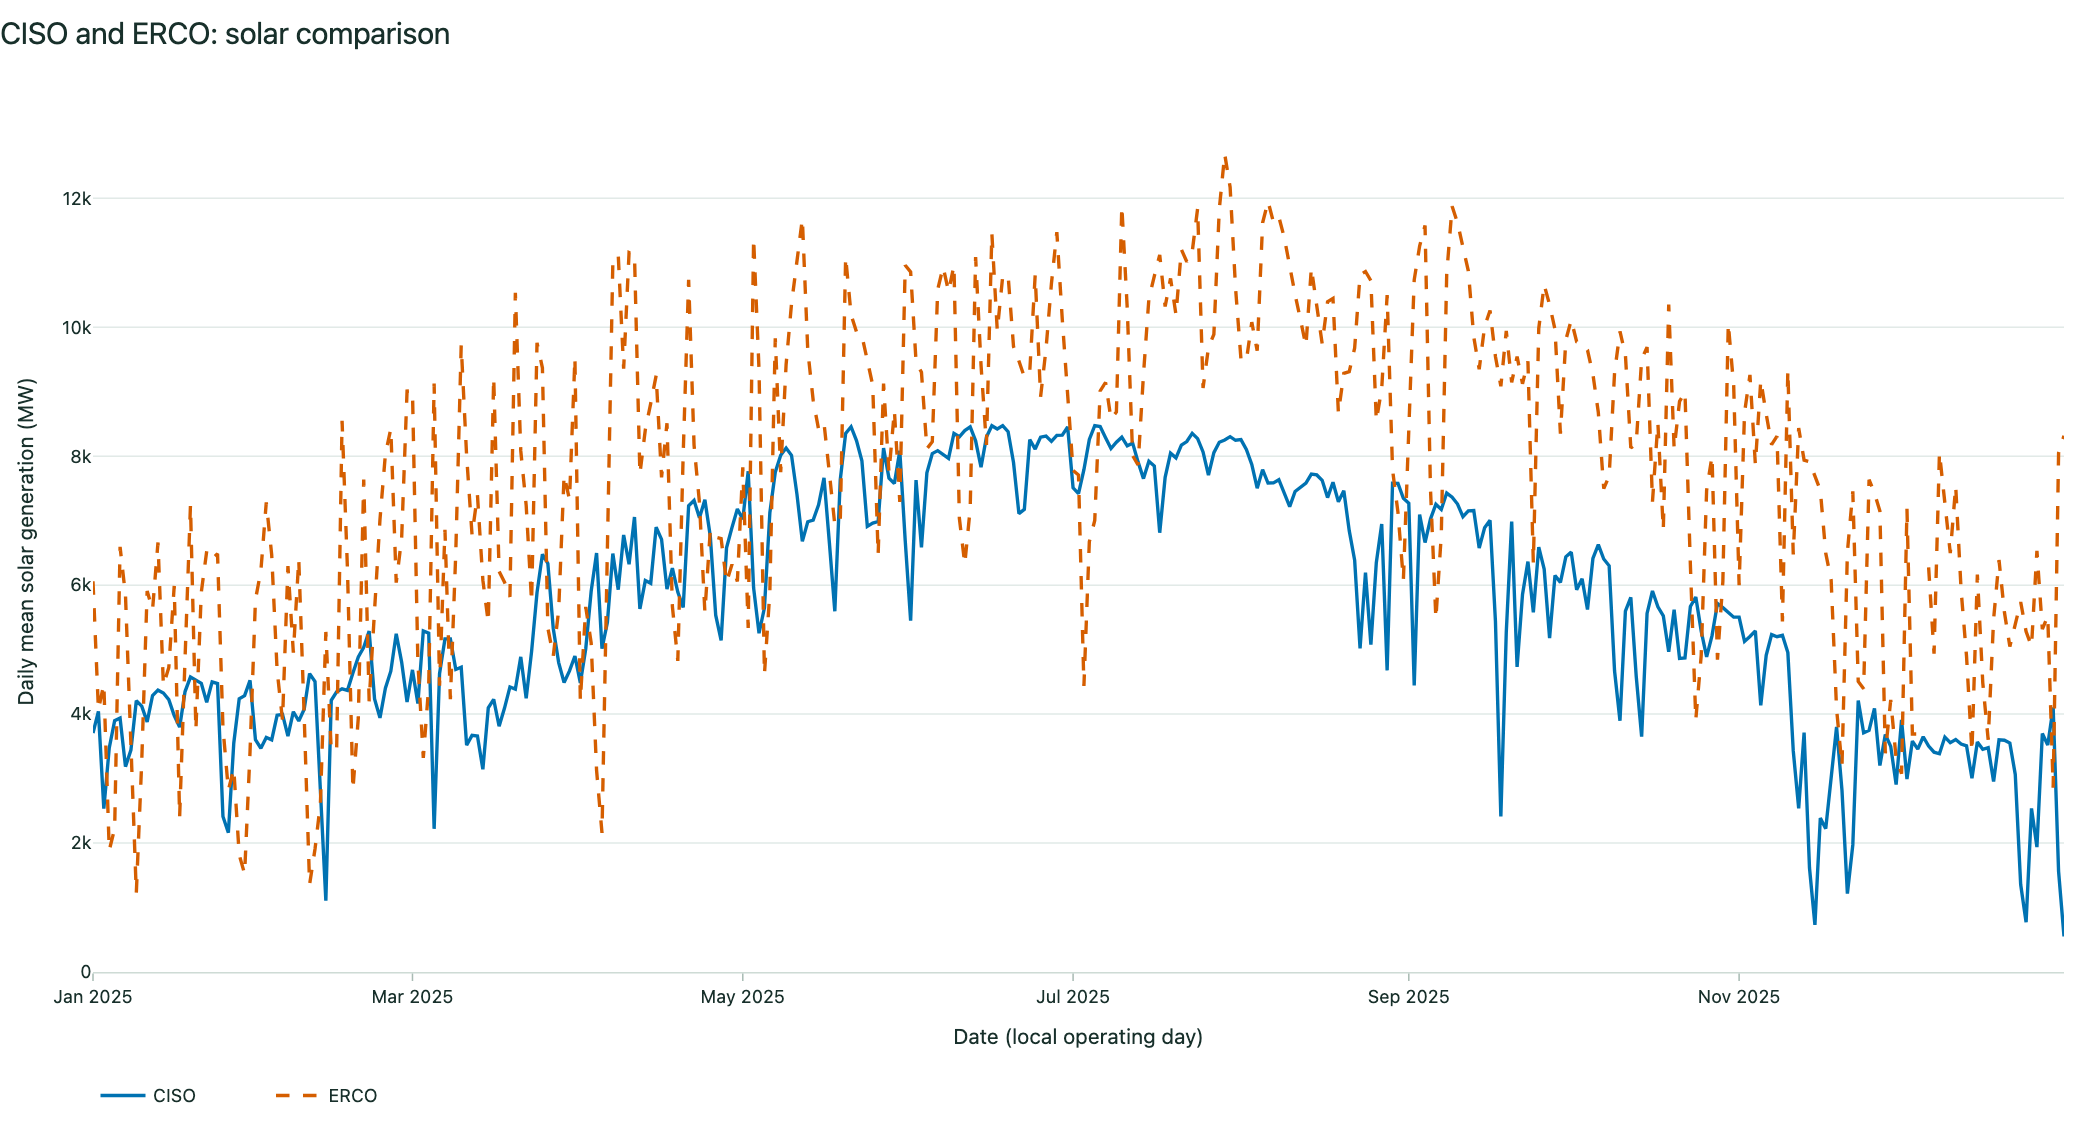
\includegraphics[width=\textwidth]{view-4-regional-comparison.png}
\caption{Matched-period CISO and ERCO solar comparison for 2025. Map points are approximate.}
\label{fig:view4}
\end{figure}

\subsection{View 5: Variability is measurable}
The hourly series is paired with mean, minimum, maximum, sample standard deviation, CV, and missing-hour cards. For CISO solar in 2025, mean output is 5,667.9 MW, maximum 18,912 MW, sample standard deviation 6,818.2 MW, and CV 1.203.
\begin{figure}[H]
\centering
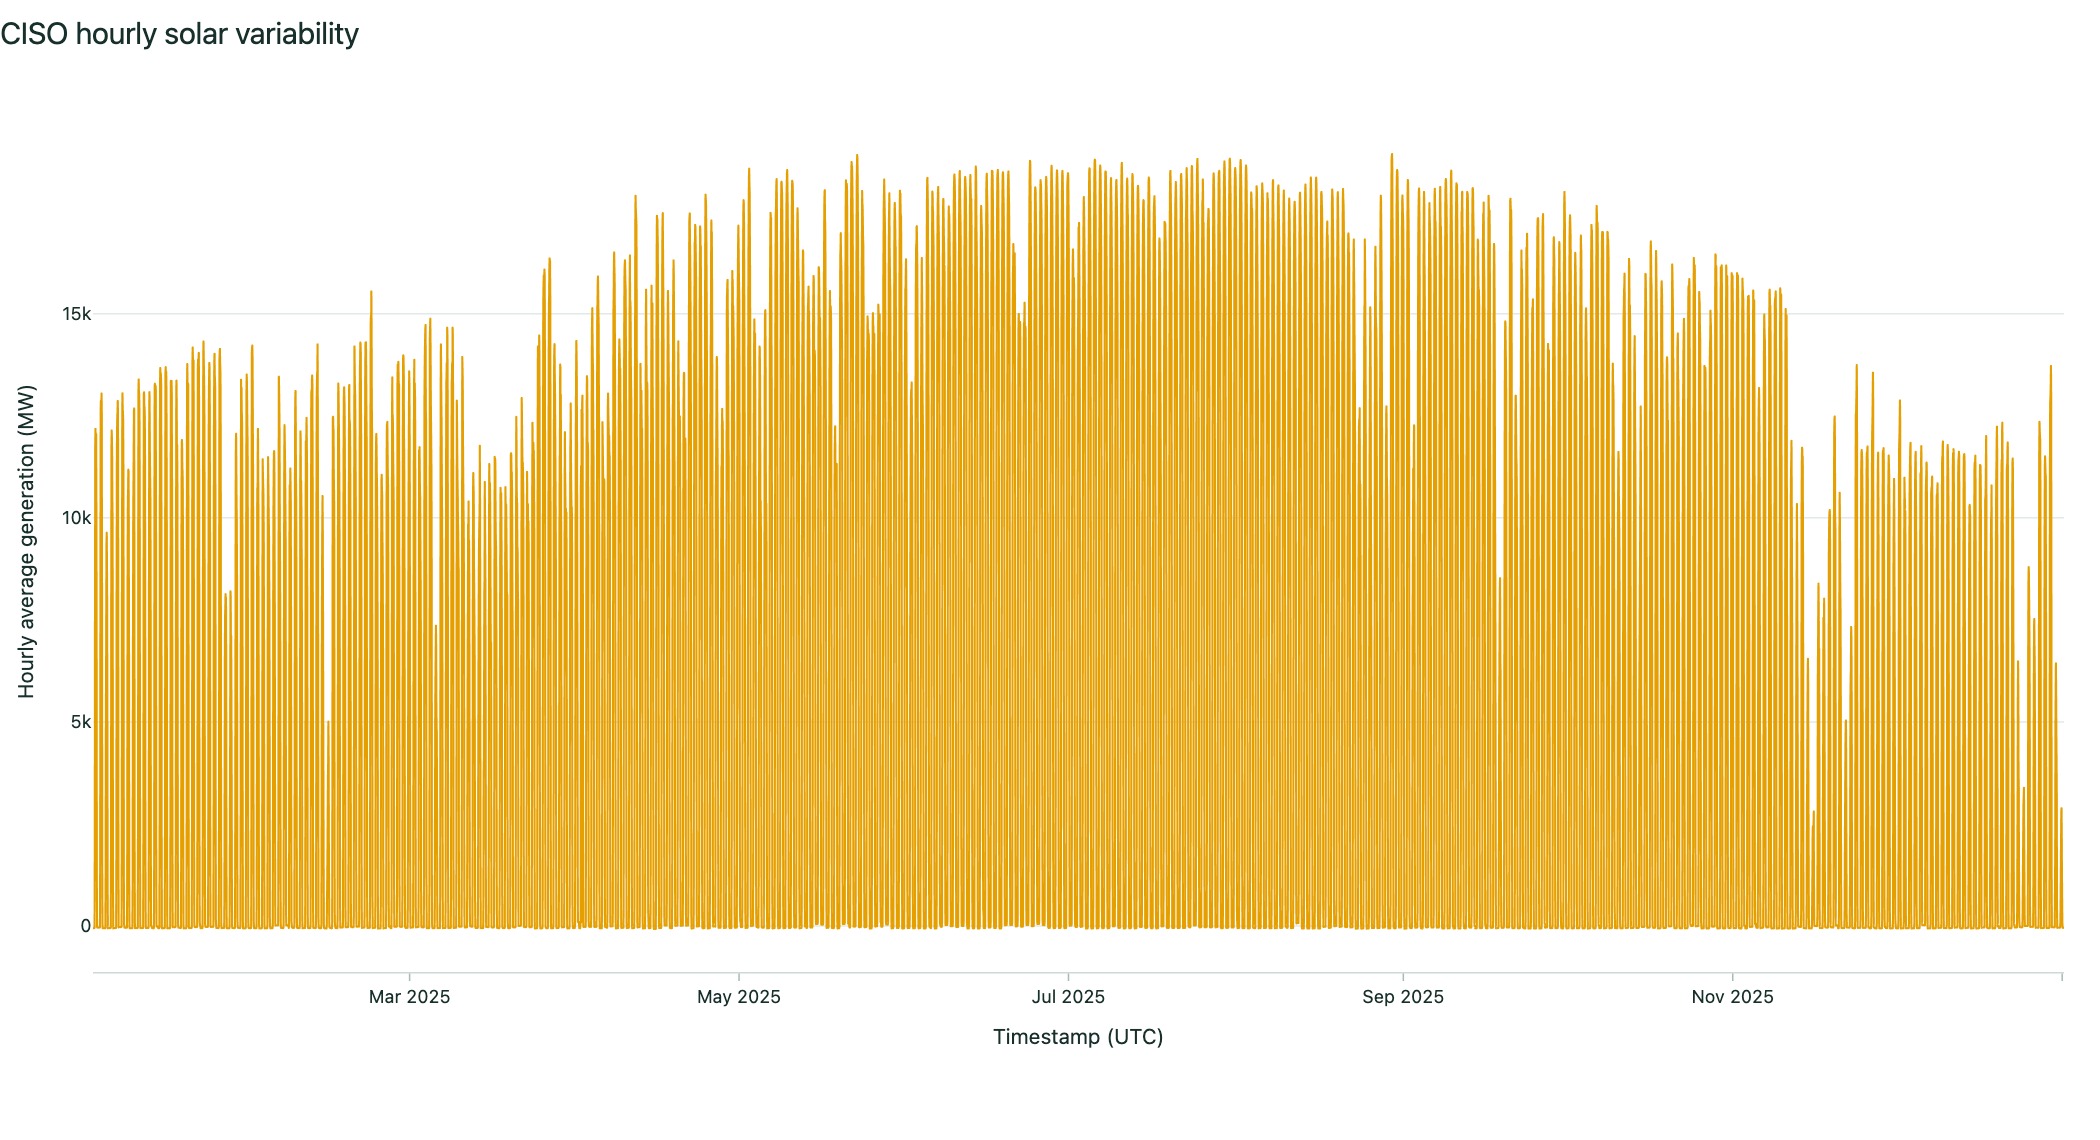
\includegraphics[width=\textwidth]{view-5-variability.png}
\caption{Hourly CISO solar variability in 2025.}
\label{fig:view5}
\end{figure}

\subsection{View 6: A portfolio can smooth the signal}
The final view stacks selected daily-mean sources, adds their combined total, and compares source and portfolio CVs. For CISO, solar CV is 1.203, wind CV 0.595, hydropower CV 0.463, and combined-portfolio CV 0.590. The portfolio is steadier than solar and wind individually but \textbf{not} steadier than hydropower.
\begin{figure}[H]
\centering
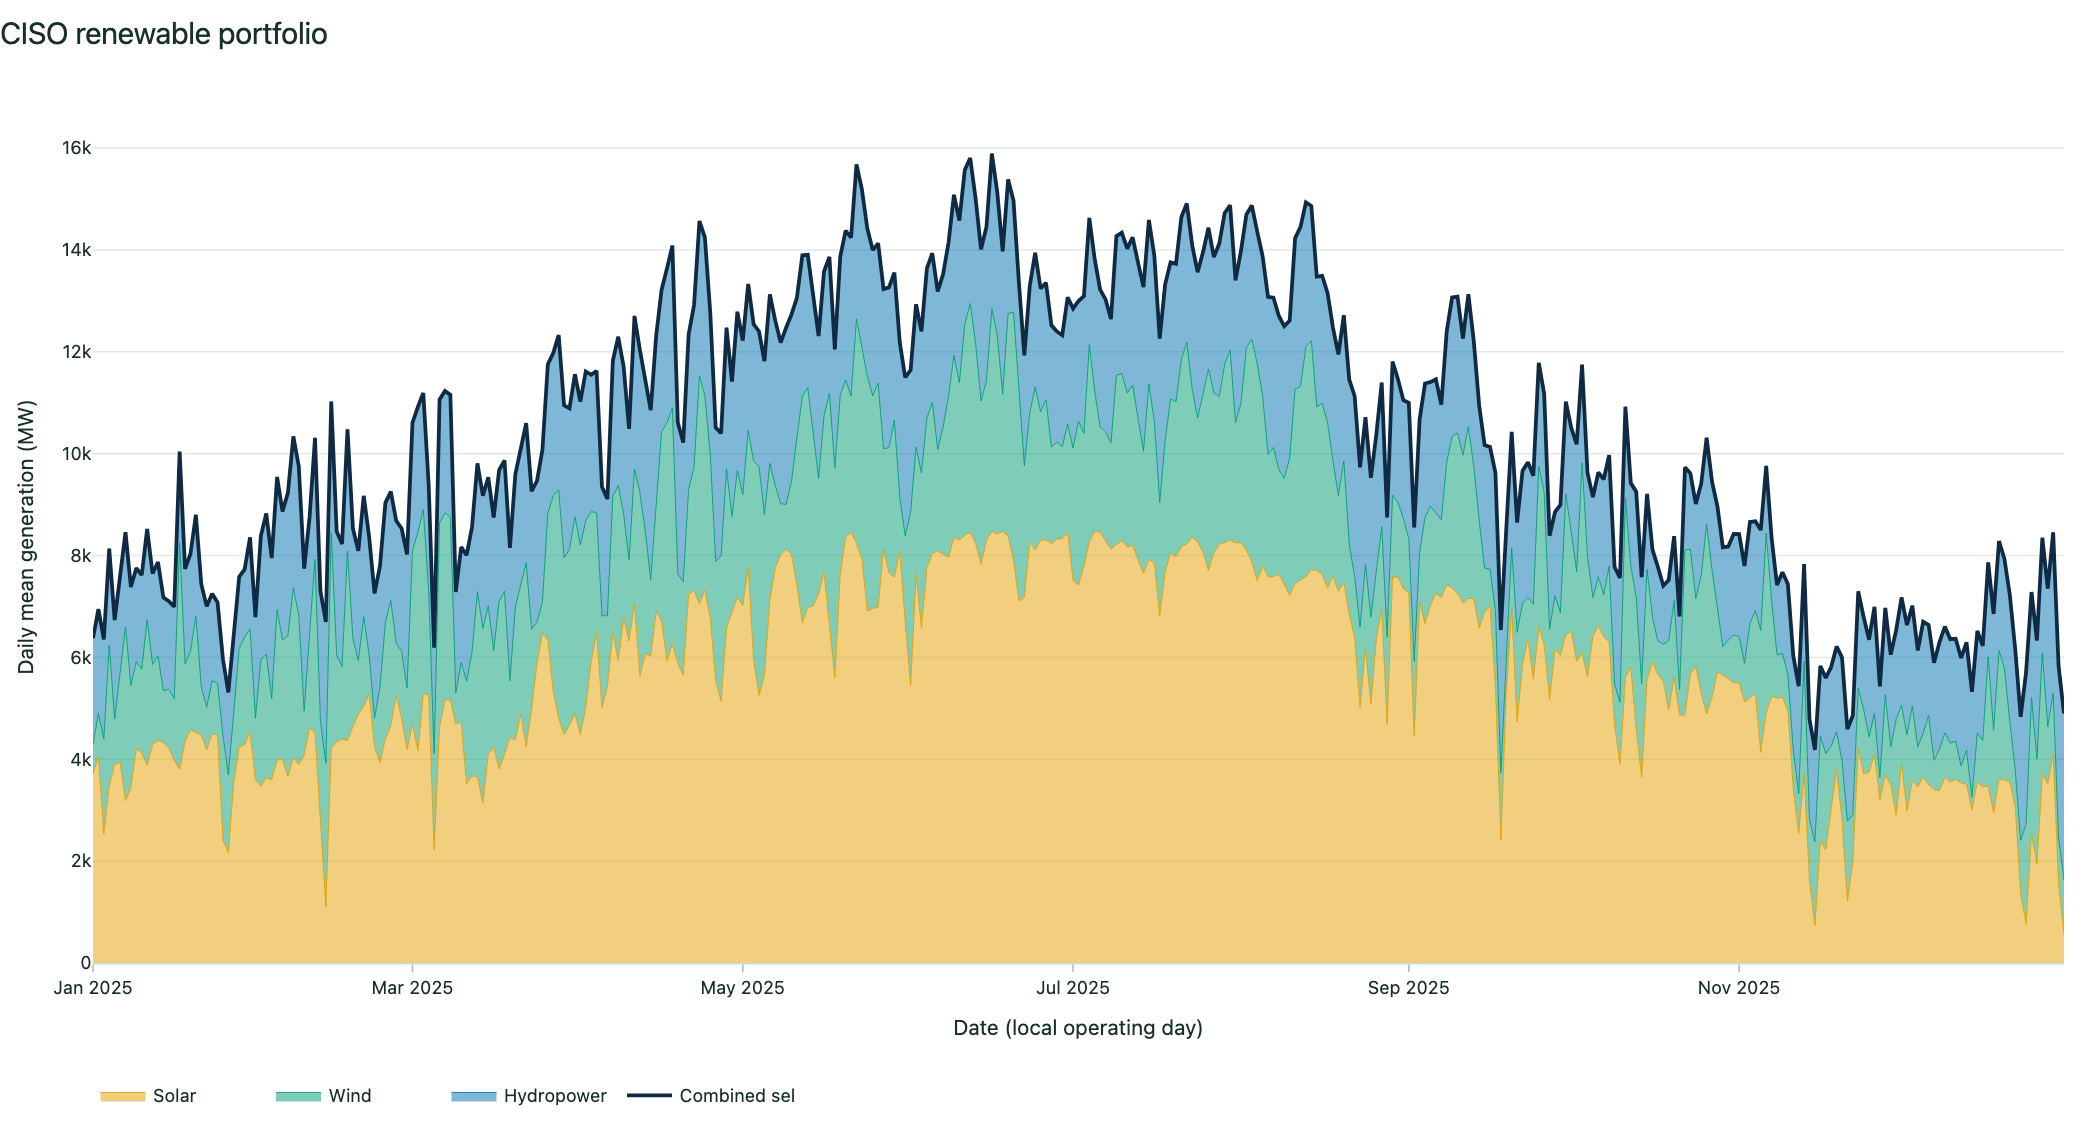
\includegraphics[width=\textwidth]{view-6-portfolio.png}
\caption{CISO renewable portfolio and companion CV comparison for 2025.}
\label{fig:view6}
\end{figure}

\section{Findings Grounded in 2025 Metrics}
\begin{table}[H]
\centering
\caption{Annual renewable metrics by balancing authority.}
\label{tab:annual}
\small
\begin{tabular}{lrrrr}
\toprule
Authority & Renewables (MWh) & Net generation (MWh) & Share & Peak (MW) \\
\midrule
CISO & 90,818,880 & 186,319,360 & 48.744\% & 24,667 \\
ERCO & 182,820,752 & 486,447,808 & 37.583\% & 46,253 \\
NYIS & 31,137,284 & 132,499,112 & 23.500\% & 6,298 \\
PJM  & 72,299,296 & 875,841,408 & 8.255\% & 22,158 \\
\bottomrule
\end{tabular}
\end{table}

\begin{table}[H]
\centering
\caption{Mean renewable output and monthly renewable-share range.}
\label{tab:means}
\small
\begin{tabular}{lrrr}
\toprule
Authority & Mean renewables (MW) & Minimum monthly share & Maximum monthly share \\
\midrule
CISO & 10,367.452 & 35.677\% (Nov.) & 60.619\% (May) \\
ERCO & 20,927.283 & 29.462\% (Aug.) & 49.613\% (Mar.) \\
NYIS & 3,556.921 & 16.664\% (Jul.) & 30.918\% (Mar.) \\
PJM  & 8,254.286 & 6.142\% (Sep.) & 11.747\% (Mar.) \\
\bottomrule
\end{tabular}
\end{table}

ERCO has the largest renewable energy, mean, and peak among the four, but CISO has the largest renewable share. PJM produces more renewable energy than NYIS in absolute terms while its share is much lower because its net generation is much larger. CISO solar's high CV reflects its strong day/night cycle. Hydropower is the least variable CISO source by CV among the three selected renewables. Combining sources lowers CISO variability relative to solar and wind, but not below hydropower alone. Portfolio smoothing depends on covariance, source selection, region, and period.

\section{Numerical Verification and Boundary Cases}
The persisted validation report passes 10 of 11 checks. The four expected authorities each have 8,760 rows; authority/timestamp pairs are unique; hourly UTC timestamps are continuous; local operating dates remain within 2025; renewable and generation-mix arithmetic have zero mismatches; excluded storage categories remain excluded; and archive integrity and provenance pass. The required-values check \textbf{fails}: demand and net generation each have 25 missing rows, while renewables and generation mix each have \textbf{31 missing rows}.

The 21 automated tests cover application structure, callbacks, download hashing, figures, visual hierarchy, metrics, preparation, and validation. Numerical checks confirm hourly MW-to-MWh summation, adjusted/imputed/raw priority, and renewable-category inclusion. Figure checks cover independent 100\% normalization, matched date axes, selected-source routing, date filtering, and empty-data annotations. Boundary handling clamps playback, supports daylight-saving day lengths, annotates empty selections, rejects unknown portfolio sources, leaves CV undefined for zero means, preserves and counts gaps, retains negative reports, and restores all three sources on reset.

\section{Timeline and Evaluation}
\subsection{Timeline}
Repository history contains one implementation commit dated October 21, 2026, so a multi-day retrospective schedule cannot be verified. The defensible timeline is the implemented dependency sequence: acquisition and provenance; preparation and quality reporting; metric and validation generation; figure functions; Dash layout and callbacks; tests; screenshot export; browser checks; and documentation packaging. This is a workflow sequence, not a fabricated record of hours spent.

\subsection{Evaluation completed and pending}
Internal browser evaluation verified desktop and mobile rendering and exercised playback and normalized controls. The six exported screenshots provide reproducible visual evidence. Instructor feedback consisted only of \textbf{``approved,''} so there were no requested proposal corrections. A later visual review supplied screenshots showing chart titles and legends overlapping. The feedback was accepted: legends now use a dedicated bottom band, margins adapt to legend rows, long titles wrap, mobile sizing was refined, and the renewable palette now uses colorblind-safe Okabe--Ito hues. The revision passed all 21 tests and regenerated figures were inspected. A broader comprehension session remains pending; usability conclusions are therefore provisional.

\section{Contingency and Collaboration}
The presentation plan includes the verified Render deployment, a local demo, and screenshot fallback if networking or rendering fails. This is an individual project by Shazab Ali. No unverified collaborator contribution or human feedback is attributed. Reproducibility comes from versioned provenance, testable computations, generated metrics, automated tests, scripted screenshots, and scripted academic outputs.

\section{Limitations}
\begin{enumerate}
  \item EIA-930 operational reports can include revisions, negatives, missing values, and authority-specific conventions.
  \item The 31 missing renewable and generation-mix rows mean required-value validation does not fully pass.
  \item Energy sums use available one-hour observations; no additional imputation is applied.
  \item Authorities differ in size and market structure; raw MW comparisons are not capacity-normalized.
  \item Normalized charts remove magnitude and are not market share or capacity factor.
  \item The renewable definition excludes pumped and standalone storage and does not measure emissions.
  \item Map markers are approximate reference points, not authority polygons.
  \item CV is not ramping difficulty, forecast error, reliability, or causation.
  \item Portfolio smoothing depends on sources and period and is not guaranteed.
  \item One year and four authorities cannot represent all U.S.\ regions or future years.
  \item One visual review is complete, but broader target-audience comprehension testing remains pending.
  \item The free Render service can spin down, delaying its first response.
\end{enumerate}

\section{Conclusion}
The six-view sequence joins context, time, place, and variability. In 2025, ERCO has the largest renewable output while CISO has the largest renewable share. Source rhythms differ strongly, and combination can reduce relative variability without outperforming the steadiest component. The evidence is reproducible: fixed provenance, explicit equations, persisted metrics, 10 of 11 validation checks passed, disclosure of 31 renewable/mix gaps, 21 automated tests, and scripted outputs. Genuine human testing remains pending rather than being invented.

\section{Launch Instructions}
Python 3.11--3.13 is recommended. Create a virtual environment, install \texttt{requirements.txt}, run \texttt{python app.py}, and open \url{http://127.0.0.1:8050}. A production-style local process uses \texttt{gunicorn app:server}. Screenshots and the academic package can be rebuilt with \texttt{python scripts/export\_report\_figures.py} and \texttt{python scripts/build\_academic\_package.py}.

\section{AI Assistance and Verification Disclosure}
AI assistance was used to help draft and format the final report, evaluation templates, reproducible PDF script, slide deck, speaker notes, deployment configuration, and this LaTeX edition from repository evidence. It was not used as an empirical source. Every quantitative claim was checked against the processed Parquet file, generated metric and validation files, implemented equations, tests, or screenshots. The public deployment and source-code links were checked during packaging and both returned HTTP 200. Only the documented visual feedback was attributed; no additional human feedback was invented. Responsibility for final review, submission, and future human-testing records remains with Shazab Ali.

\nocite{pandas,project-repository}
\bibliographystyle{plainnat}
\bibliography{references}

\end{document}
